\begin{frame}
  \frametitle{\Glspl{PCC} convey sensitivity of \gls{DNP} group parameters to nuclear data}
  \begin{columns}
    \column[t]{0.45\textwidth}
        \begin{figure}[!ht]
                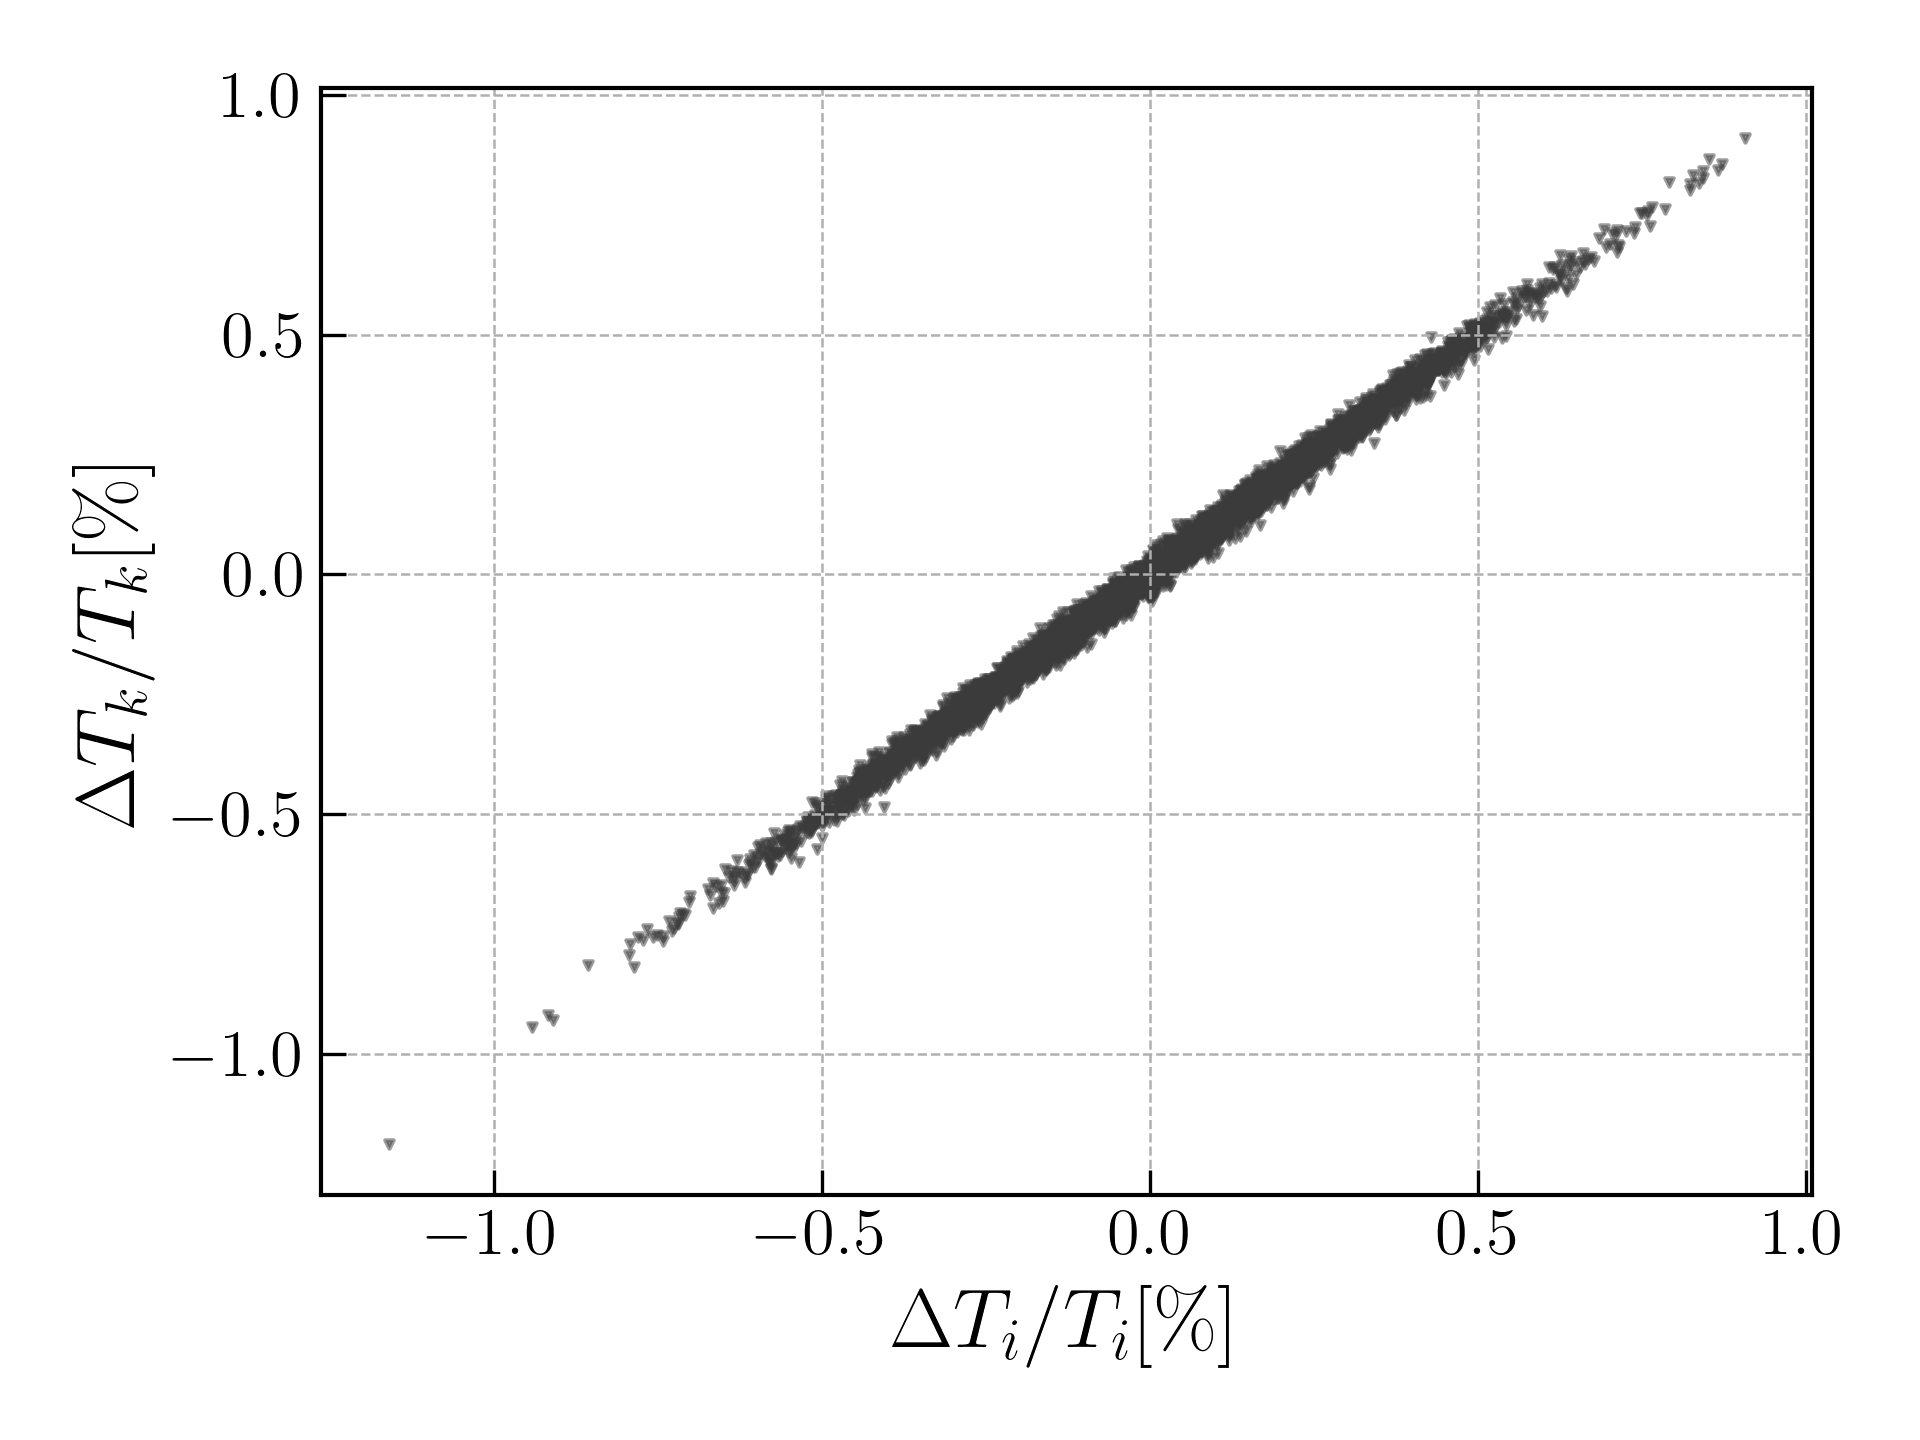
\includegraphics[width=1.0\linewidth]{../images/sens_lam_halflife_Br87_1.png} 
                \caption{\Gls{DNP} group 1 half-life variation due to half-life variation with a \gls{PCC} of 1.00.}
        \end{figure} 
    \column[t]{0.45\textwidth}
        \begin{figure}[!ht]
                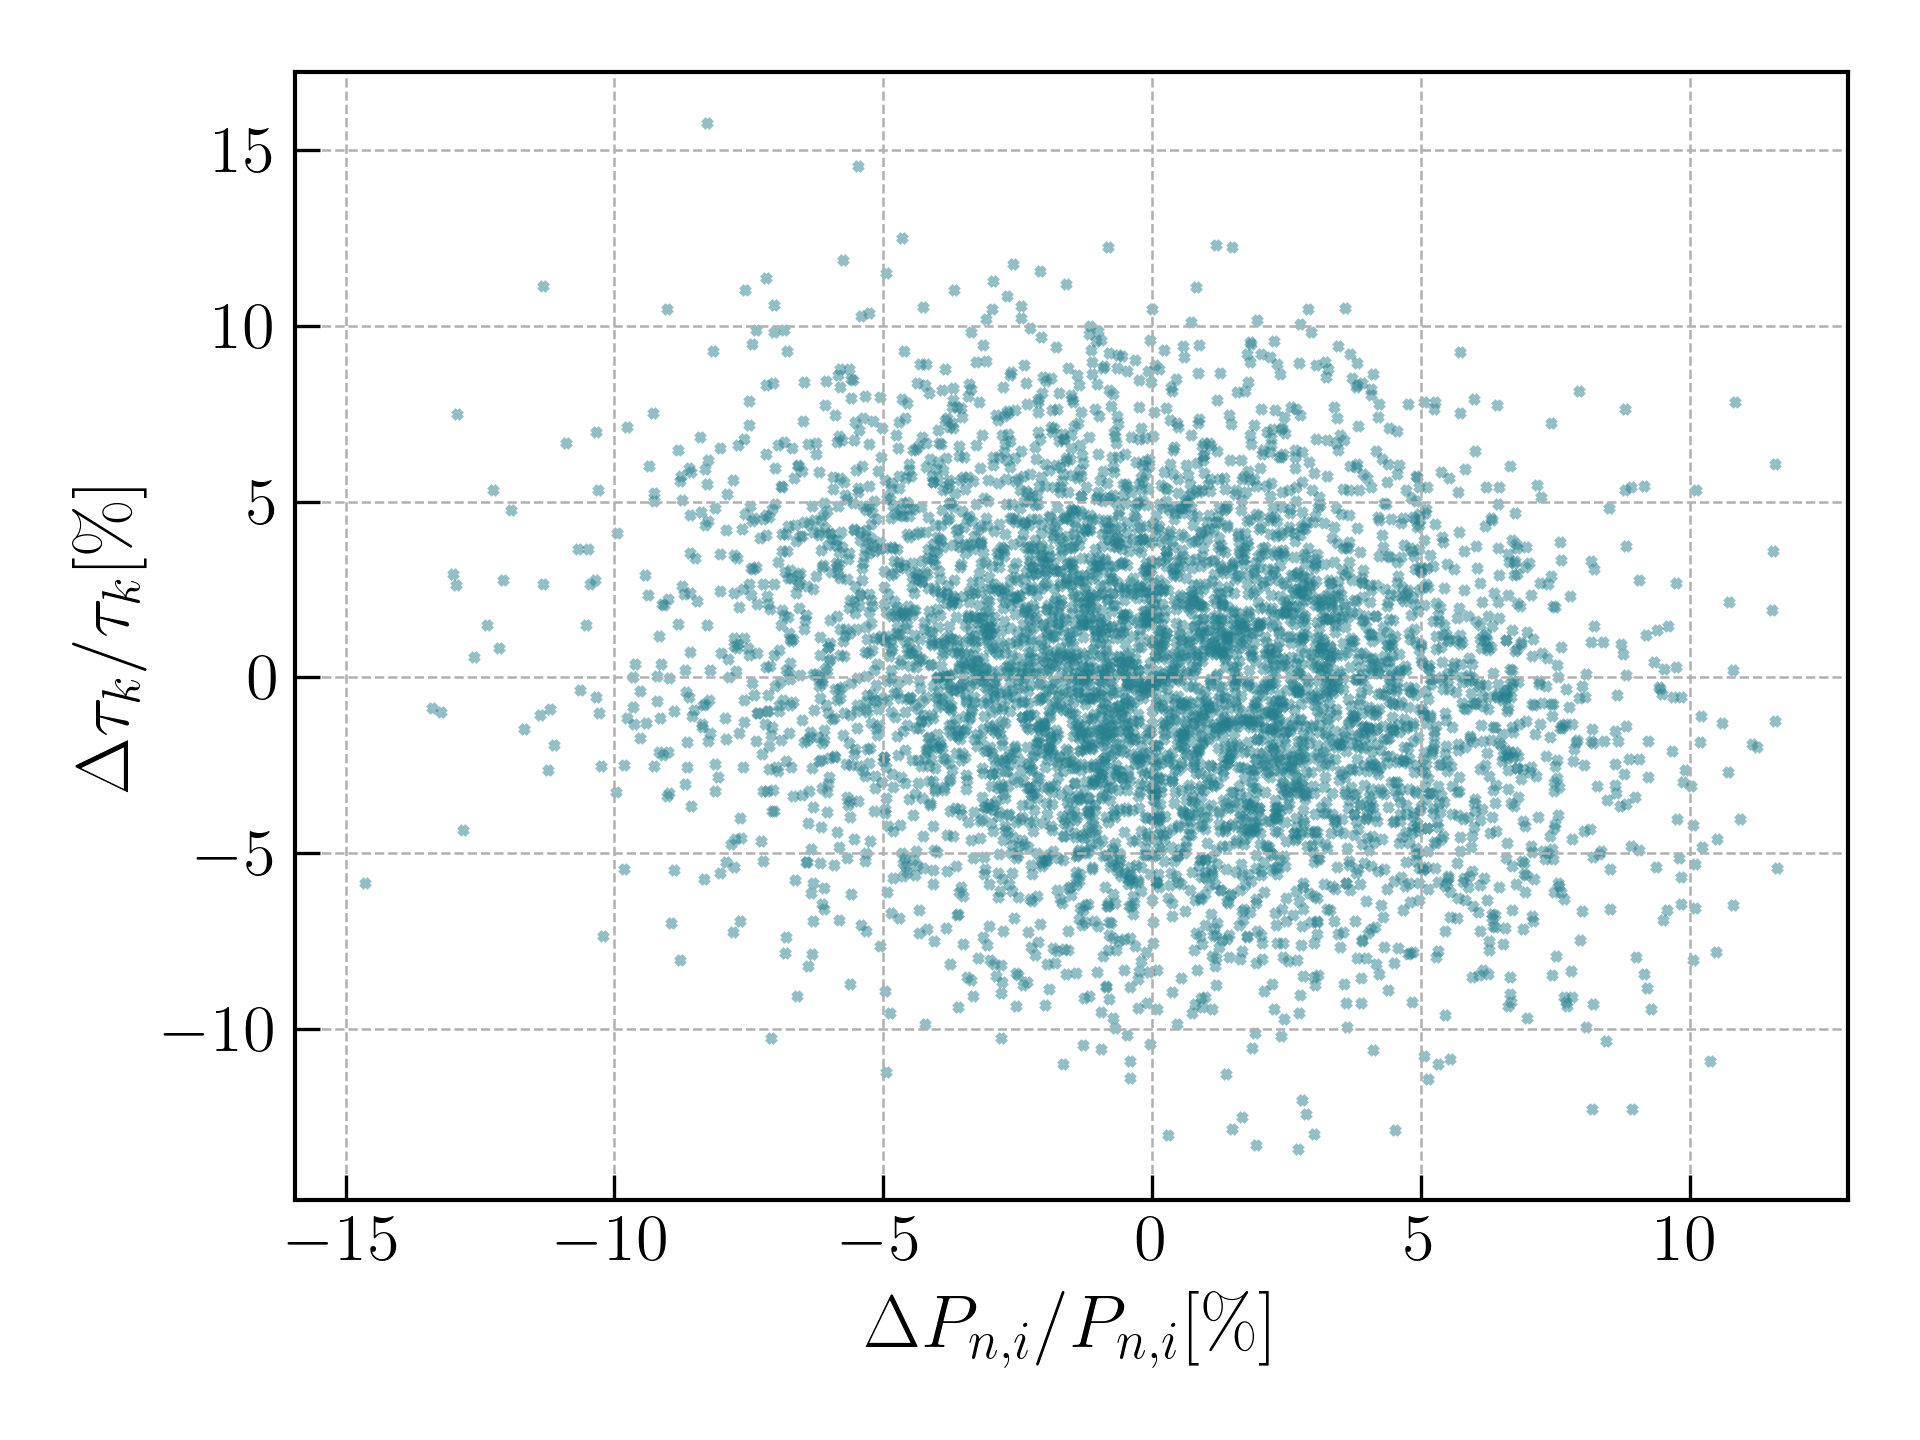
\includegraphics[width=1.0\linewidth]{../images/sens_pn_halflife_Br87_3.png} 
                \caption{\Gls{DNP} group 3 half-life variation due to emission probability variation with a \gls{PCC} of -0.19.}
        \end{figure} 
  
  \end{columns}
  \textbf{The half-life of $^{87}$Br strongly correlates to the group one half-life, while its emission probability does not strongly correlate to the group three half-life.}

\end{frame}

